\documentclass[12pt]{article}
\usepackage[utf8]{inputenc}

\usepackage{titlesec}
\titleformat{\section}[block]{\Large\bfseries\filcenter}{}{1em}{}
\titleformat{\subsection}[hang]{\bfseries}{}{1em}{}


\usepackage[margin=1in]{geometry,caption}

%IMAGES
\usepackage{graphicx}
%\graphicspath{ {/Users/ethancreagar/Documents/WorkProjects/CSUA/TexReport/Images/} }

\title{ADV Help Analysis Project}
\author{Ethan Creagar}
\date{September 2020}

\begin{document}

\begin{titlepage}
\maketitle
\end{titlepage}

\tableofcontents
\bigskip

\listoffigures
\newpage

\begin{abstract}
What is this report intended to be? I don't know. I'll fill this in later.
\end{abstract} \hspace{10pt}

%EXAMPLE OF HOW TO USE SECTIONS AND SUBS
%\section{Hello}
%\subsection{Subsection}
%\subsection{Subsection 2}
%\section{Go on}
%\subsection{Subsection 3}
%\end{document}

\section{Overview}

\subsection{How Many Tickets Have we Received/Completed?}

Since 2016, ADV Help has received a total of 13,846 emails. Of these emails, 5,568 were unique (indicated by the subject line not starting with "RE:" and not including informational tickets). We Of these 5,568 unique tickets, we have completed an estimated 5313, a percentage of $95.42 \pm 5$ \%. Note that this percentage is has an error margin. This is due to tickets being marked "Done" twice in different spots. Since our analysis sorts by Subject Line, these may be counted twice in the Done group. This has grown steadily over time, with 2020 being our most emailed month (so far, on average) and March of 2020 being the most emailed month. This is unsurprising due to the drastic technology adjustments made due to quarantine.

\begin{figure}[h]
    \centering
    \captionsetup{width=.8 \linewidth}
	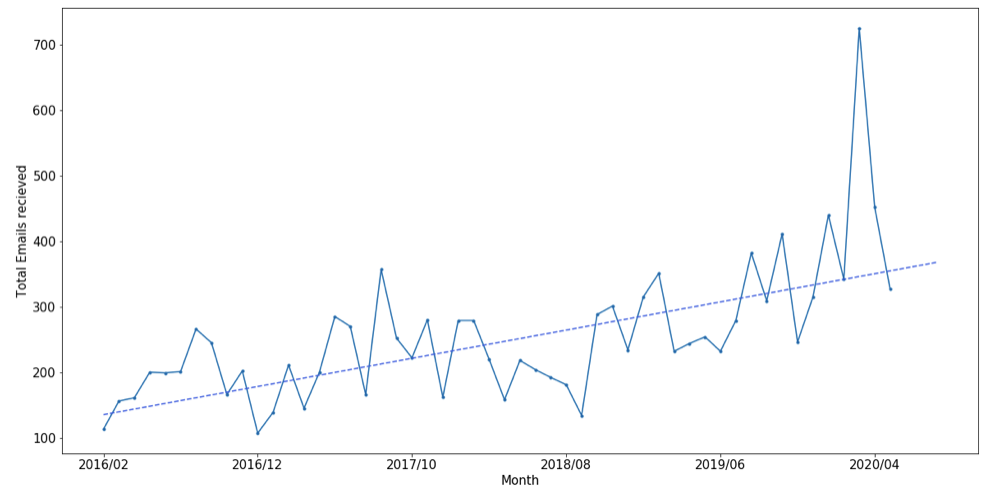
\includegraphics[width=13cm, height=6cm]{Images/EmailsOverTime.png}
	\caption[Emails Received Per Month]{With an intercept of 135.2, we expect to receive an additional 4.3 emails per month on average.}
\end{figure}

\newpage

\section{New}

\end{document}